%[prl] it will mess up section numbers but puts our emails in the bibliography section
%[eqsecnum] Number equations by section
%
%
%\documentclass[prd,preprint,letterpaper]{revtex4}
\documentclass[aps,prb,twocolumn,superscriptaddress]{revtex4-1}

\usepackage{graphicx}	% this is the up-to-date package for all figures
\usepackage{amssymb}	% for math
\usepackage{verbatim}	% for the comment environment
\usepackage{color}
\usepackage{subcaption}	% for sub-captions on side-by-side figures
\usepackage{float}		% allows use of 'H' command
\usepackage{tikz}		% lets you draw: graphics, flowcharts, pie graphs, etc
%\usepackage[final]{pdfpages}	% allows extern pdf to be included

%%%
% For fancy section references
%%% 
% This allows you to use '\cref{}' to reference sections with the symbol
\usepackage{cleveref}
\crefname{section}{\S}{\S\S}%{§}{§§}
%% Usual (decimal) numbering
\renewcommand{\thesection}{\arabic{section}}
\renewcommand{\thesubsection}{\thesection.\arabic{subsection}}
\renewcommand{\thesubsubsection}{\thesubsection.\arabic{subsubsection}}
%% Fix references
\makeatletter
\renewcommand{\p@subsection}{}
\renewcommand{\p@subsubsection}{}
\makeatother
%%%%%
%%%


\def\deg{\ifmmode^\circ\else$^\circ$\fi}
\def\arcsec{\ifmmode^{\prime\prime}\else$^{\prime\prime}$\fi}
\def\arcmin{\ifmmode^{\prime}\else$^{\prime}$\fi}
\def\solar{\ifmmode_{\mathord\odot}\else$_{\mathord\odot}$\fi}
\def\earth{\ifmmode_{\mathord\oplus}\else$_{\mathord\oplus}$\fi}

%%%
% Change labeling of figures and tables - currently it defaults to 'FIG.'
%%%
\renewcommand{\figurename}{Figure}
\renewcommand{\thefootnote}{\roman{footnote}} %for footnotes in roman numerals
%\renewcommand{\thetable}{\Roman{table}}

\bibliographystyle{apsrev}


% these are some custom control of the page size and margins
% \topmargin= 0.2in  % these 1st two may be needed for some computers
% \textheight=8.75in
\textwidth=6.5in
%\oddsidemargin=0cm
%\evensidemargin=0cm


\begin{document}

\title{Assassinating ASASSN:\\ Supernovae Identification Using ATLAS Data}

\author{Corey Mutnik}
\email{cmutnik@hawaii.edu}
\affiliation{Department of Physics \& Astronomy, \\
University of Hawaii at Manoa,\\
2505 Correa Rd, Honolulu, HI, 96822, USA}
\altaffiliation{ASTR 399}



% \section is used to start a new one with a heading
\begin{abstract}
Using current data collection and reduction techniques, we plan to 
identify supernovae (SNe) faster and fainter than the All-Sky Automated 
Survey for Supernovae (ASASSN) team is able to. 
%With a declination limit of $-30^{\circ}$
We expect to identify all SNe, with $m>17.5$ and declinations above $-30\deg$, 
before ASASSN is able to.\\
%For SNe with $m>17.5$ and declination (dec) $>-30\deg$
%We expect to identify all supernovae (SN) above a declination of $-30\deg$, with $m>17.5$, before ASASSN is able to.\\
{\bf m$>$17.5 --OR-- $m>17.5$}\\
{\bf 17.5 (0.5mag) --OR-- 18 (1mag) fainter...which is it?}\\
{\bf not emphasis on Type Ia supernovae?}
\end{abstract}


\maketitle    



\section{Introduction}
{\bf Supernova (SN)}\\
{\bf check plurality throughout paper: SN or SNe}\\
Supernovae (SNe) identification using data collected by ATLAS.\\

%%%%%%%%%%%%%%%%%%%%%%%%%%%%%%%%%%%%%%%%%%%%%%%%%%%%%%%%%%%%%%%%%%%%%%%%%%%%%%%%%%%%%%%%%%%%%%%%%%%%
%%%%%%%%%%%%%%%%%%%%%%%%%%%%%%%%%%%%%%%%%%%%%%%%%%%%%%%%%%%%%%%%%%%%%%%%%%%%%%%%%%%%%%%%%%%%%%%%%%%%
%%%
% Input general notes and things that need to be fixed / addressed
%%%
\input general_notes.tex
%%%%%%%%%%%%%%%%%%%%%%%%%%%%%%%%%%%%%%%%%%%%%%%%%%%%%%%%%%%%%%%%%%%%%%%%%%%%%%%%%%%%%%%%%%%%%%%%%%%%
%%%%%%%%%%%%%%%%%%%%%%%%%%%%%%%%%%%%%%%%%%%%%%%%%%%%%%%%%%%%%%%%%%%%%%%%%%%%%%%%%%%%%%%%%%%%%%%%%%%%



\iffalse
 \section{Observations}
 \section{Data Processing}
\fi


\section{Collected Data}

%\section{ASASSN Breakdown}
\subsection{ASASSN Data}
\begin{itemize}
	%\item{} {\bf Where'd it come from}
	%\item{} {\bf ASASSN specs}
	\item{} {\bf ASASSN or ASAS--SN}
	%\item{} {\bf images have 7.8\arcsec pixels}
\end{itemize}


\indent The All-Sky Automated Survey for Supernovae (ASASSN) group 
collects data using eight $14~cm$ telescopes. Each night, these  
telescopes are able to cover roughly $20,000~deg^{2}$, reaching 
down to $\sim$17th magnitude.
%{\bf reword}\\
These eight telescopes are split evenly between two sites.
The first telescope array is located on Haleakala and began 
collecting data in December 2013. In July 2015, the second %telescope 
array became operational at the LCOGT Cerro Tololo station. 
This allows ASASSN to detect SNe in both hemispheres.
{\bf Cite using footnote.--OR--~\cite{asn_data}}
%~\footnote{http://www.astronomy.ohio-state.edu/~assassin/index.shtml}

\indent Using 400mm f/2.8G Nikon lenses allows for a large field of 
view. ProLine PL230 CCD cameras are used as detectors. Detection of 
%Transients are detected using image subtractions. 
transients is made possible using image subtraction. With images 
having 7.8\arcsec pixels, ASASSN relies on volunteers collecting  
confirmation images with larger telescopes.
{\bf Cite using footnote.}

%data collected by two 14--cm telescopes\\
%one at Haleakala, the other at the LCOGT Cerro Tololo station.\\
%first guy started in December 2013...second came online in July 2015.\\
%these two currently cover roughly 20,000~$deg^{2}$ a night\\
%down to 17th mag\\
%they eventually plan to survey the entire sky, every night, down to 17th mag, using 16 scopes at 4 diff sites\\
%\footnote{http://www.astronomy.ohio-state.edu/~assassin/index.shtml}


% OLD plots as single
 %\begin{figure}[H]%[h!]
 %  \begin{center}
 %\centerline{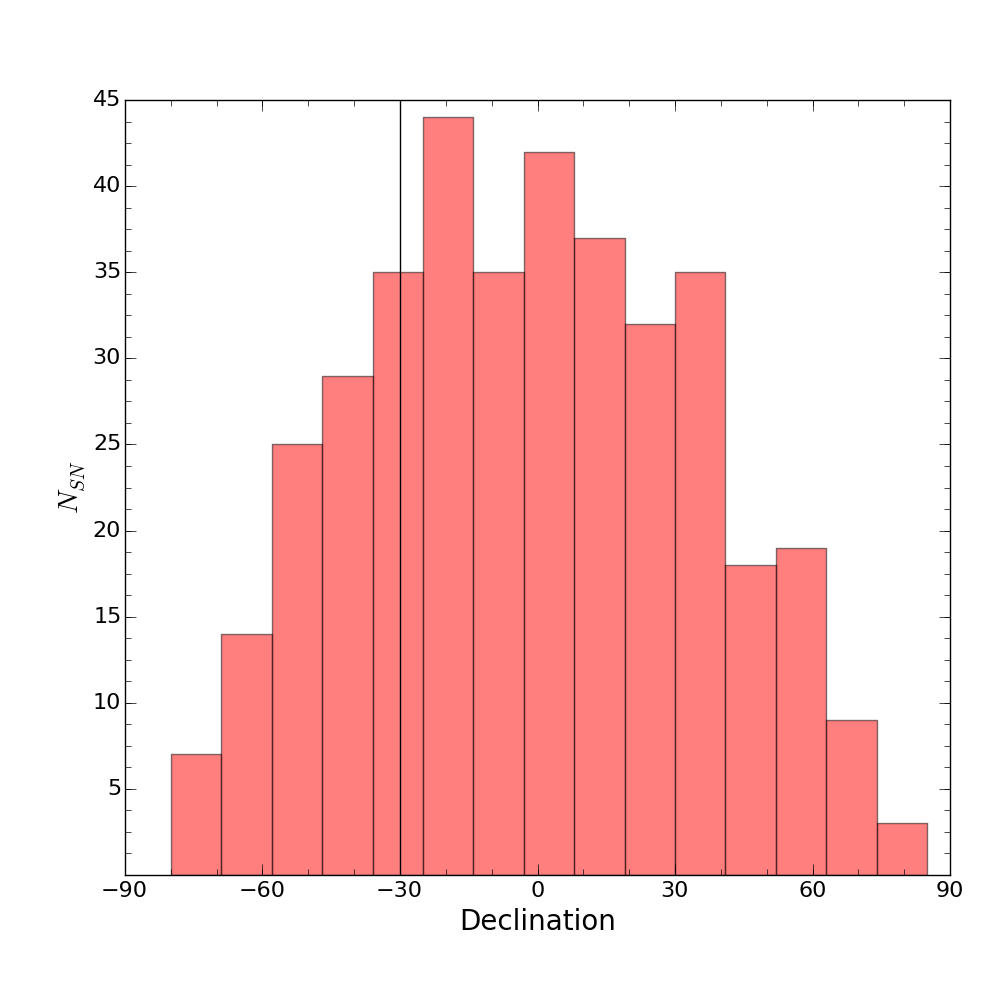
\includegraphics[width=3.35in]{figures/dec_histo_step10.png}}
 %\caption{\it \small{ASASSN SN sorted by their declination. The vertical line at $-30^{\circ}$ indicates the lower limit on ATLAS observations. \label{fig:asn_dec}}}
 %  \end{center}
 %\end{figure}
 %\begin{figure}[H]%[h!]
 %  \begin{center}
 %\centerline{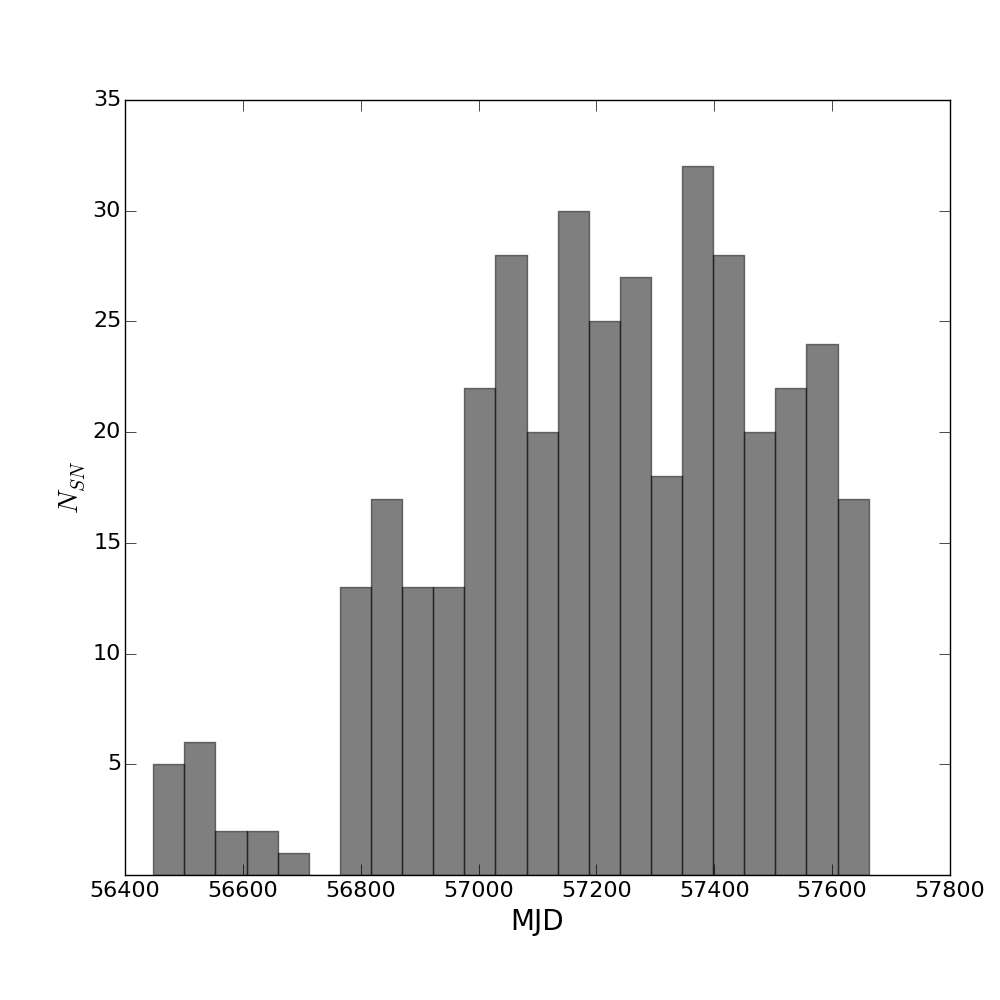
\includegraphics[width=3.35in]{figures/mjd_histo_step50.png}}
 %\caption{\it \small{Discovery date of ASASSN SN. \label{fig:asn_mjd}}}
 %  \end{center}
 %\end{figure}
 %~[MAKE THIS A DUAL FIGURE: (a) (b)]

\begin{figure*}
	\centering
	\begin{subfigure}{.5\textwidth}
	  \centering
	  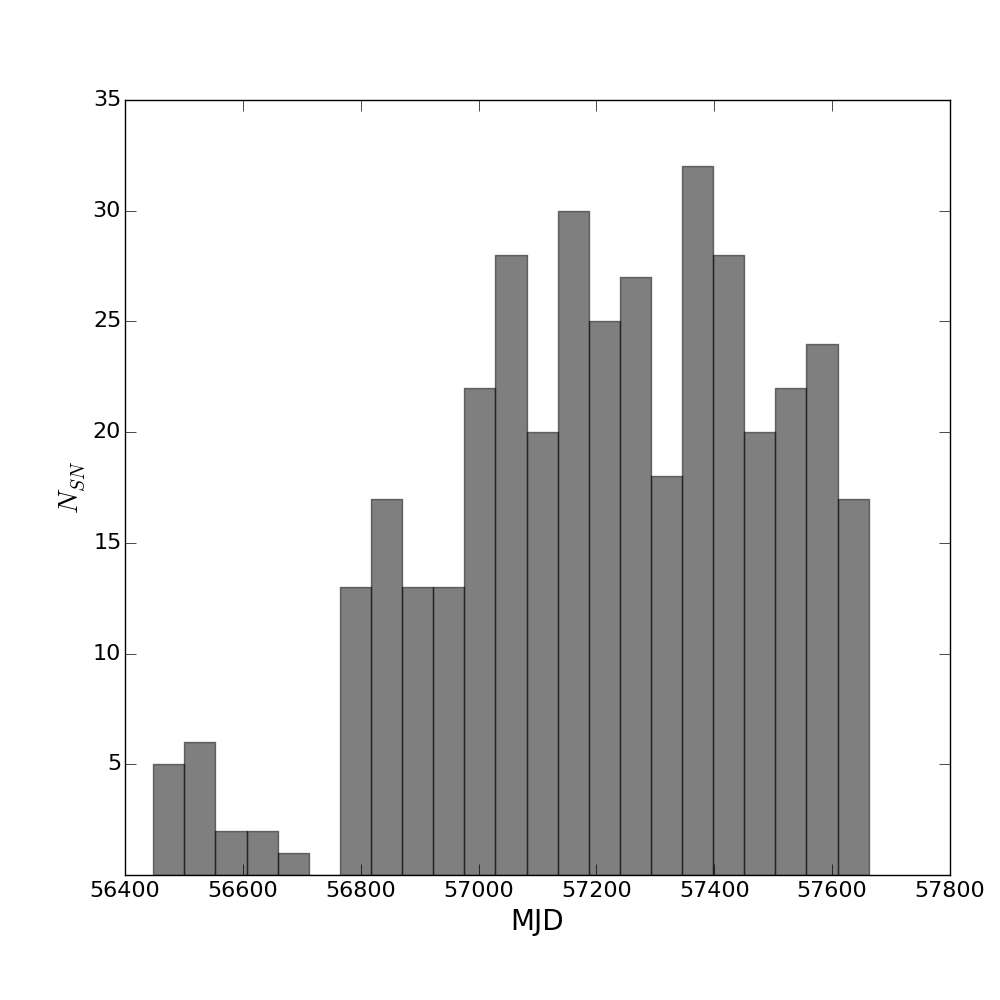
\includegraphics[width=1\linewidth]{figures/mjd_histo_step50.png}
		\caption{\it \small{ }}
		\label{fig:mjdhist}
	\end{subfigure}%
	\begin{subfigure}{.5\textwidth}
	  \centering
			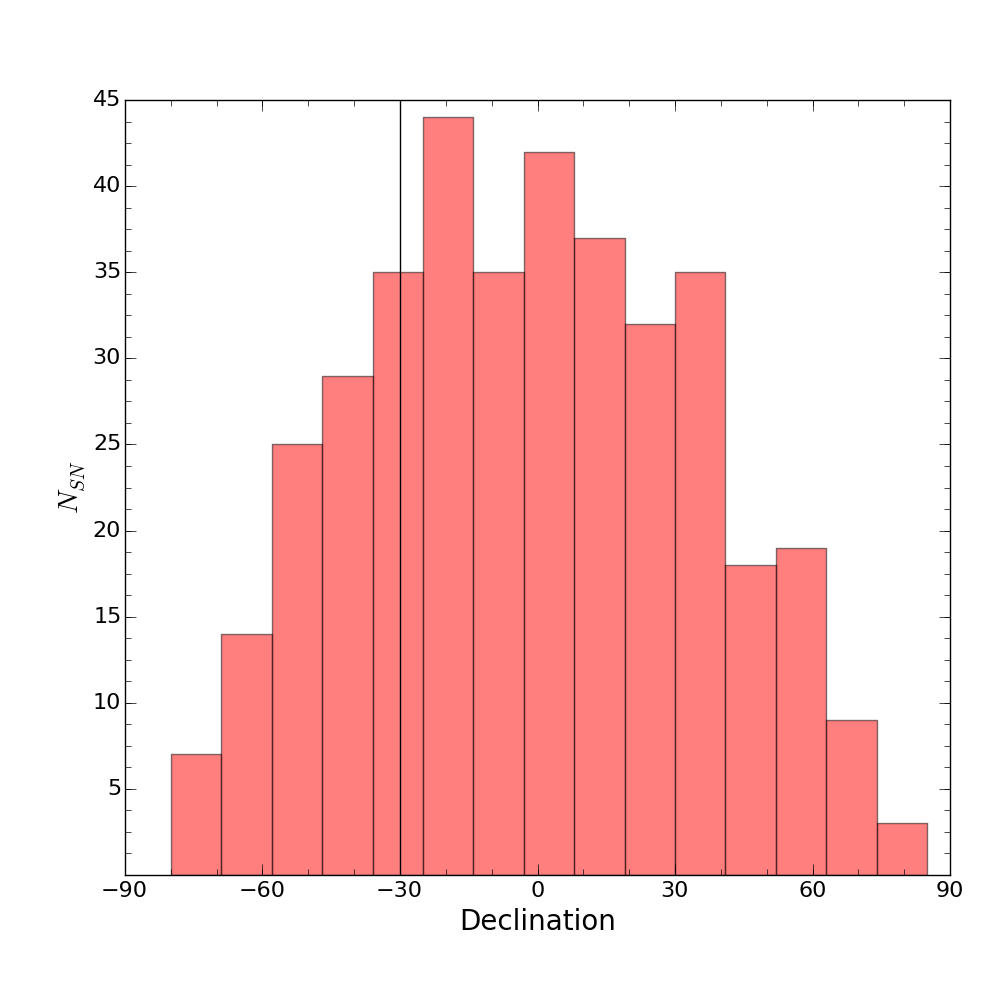
\includegraphics[width=1\linewidth]{figures/dec_histo_step10.png}
		\caption{\it \small{ }}
		\label{fig:dechist}
	\end{subfigure}
	\caption{\it \small{SN discovered by the ASASSN project.  Panel `(a)' shows ASASSN SN discovery dates.  Panel `(b)' is ASASSN data, binned by dec. The vertical line at $-30^{\circ}$ indicates the lower limit on ATLAS observations.}}
	\label{fig:asnhist}
\end{figure*}


\subsection{ATLAS}
ATLAS PathFinder 2 Observations
\begin{itemize}
	\item{} ATLAS specs
	\item{} how data was collected
	\item{} how *.diff.fz is made - subtract wallpaper from reduced data
	\item{} how *.ddt is made
	\item{} what is starrat
	\item{} \cite{ATLAS_data}
	%\item{} reduced data became good around 57364
\end{itemize}

ATLAS began collecting data in June 2015. Reduction methods 
are always being refined and improved. Data reduced before 
December 2015 is not trusted, when ATLAS became truly operational.\\
%Although ATLAS came on-line in June 2015, data reduced before December 2015 is not trusted. 
{\bf REWORD}


\section{Procedure}
%\begin{enumerate}
	%\item{} find asn SN in atlas data
	%\item{} use asn SN to restrict ATLAS classification variables
	%\item{} manually inspect results for SN classification
%\end{enumerate}
{\bf want to make input sections subsections under this section?}
{\bf quantify: how many objects are potentially SNe before class.var. restriction, how many after\\
$0.9 < starrat < 1.2$\\}
%{\bf [check date]\\}
{\bf possibly include starrat figure\\
use DS9 image?\\
~~~remake it\\
~~~identify exact dates shown by tiles}

\indent In order to assassinate ASASSN, 
%\indent Before assassinating ASASSN became a possibility,
it was necessary to show that ATLAS had the potential to find all of ASASSN discovered SNe. 
%%To refine our SNe search, a trial set was needed. SNe ASASSN team has been 
To do this, a list of all ASASSN discovered SNe was obtained~\cite{asn_data}. 
{\bf [--OR-- cite website using footnote]}
By October 11, 2016 
ASASSN has reported discovering 385 SNe. Many of these 
objects were reported before ATLAS was operation. Object cuts are discussed 
in~\cref{sec:expobs}. Once the data was properly culled, the remaining SNe 
%served as a {\bf sanity test / validity check}. {}
were found in observations made by ATLAS. 
One such SN is shown in Figure~\ref{fig:ds9_ASASSN-16ke}.
Finding these SNe in the ATLAS 
data allowed restrictions to be placed on classification variables, drastically 
reducing the number of potential SNe candidates. With such a restricted object 
list, visually examination is able to be used in identifying SNe.\\ 
%These identified SNe allowed for the restriction of ATLAS classification variables.


\begin{figure}[H]%[h!]
   \begin{center}
 \centerline{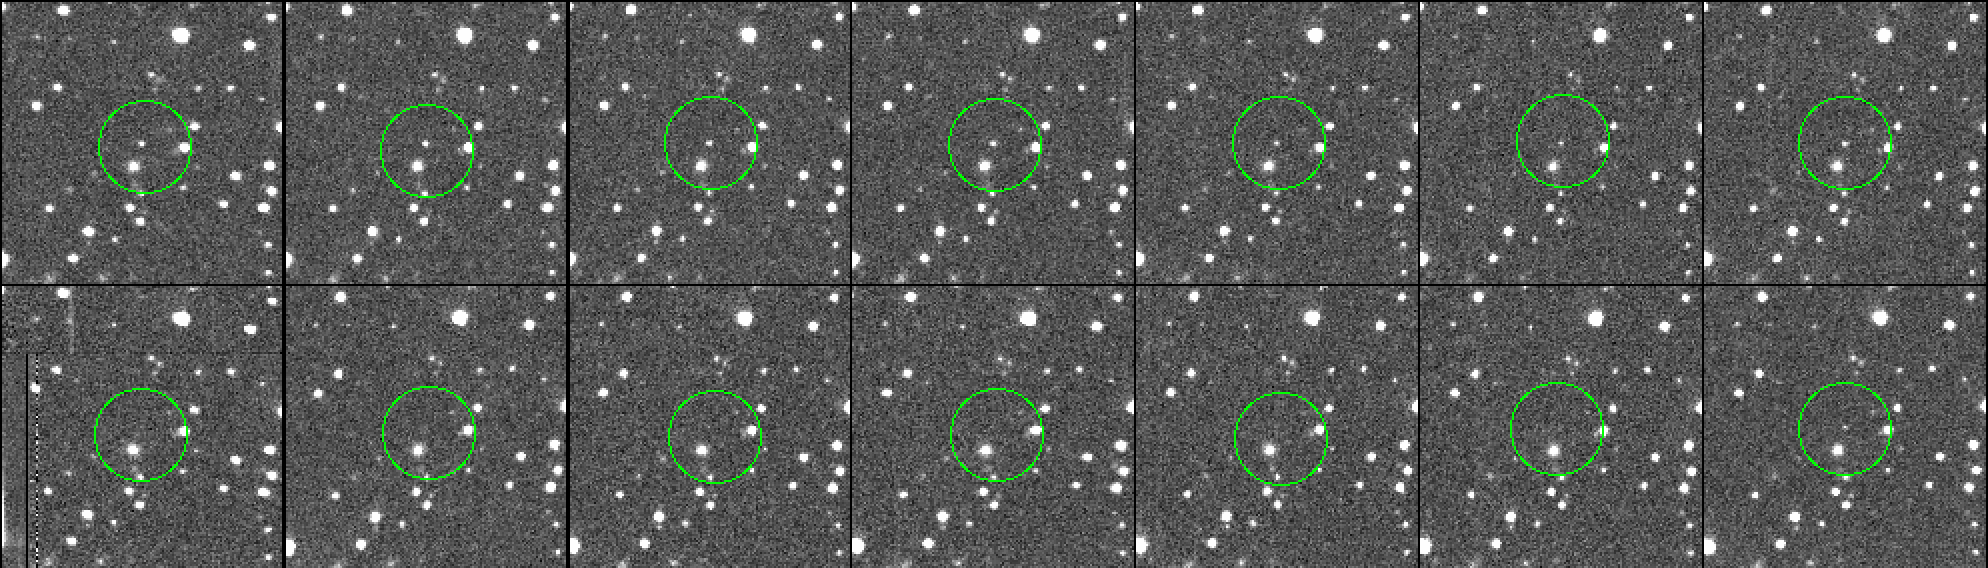
\includegraphics[width=3.35in]{figures/ds9_asn16ke.png}}
 \caption{\it \small{Each tile shows a different ATLAS observation of the SN ``ASASSN-16ke''. The SN is enclosed by a green circle, to show its exact location. \label{fig:ds9_ASASSN-16ke}}}
   \end{center}
\end{figure}
{\bf comment on lower panel showing ATLAS obs before SN appeared in fig~\ref{fig:ds9_ASASSN-16ke}?}



%%%%%%%%%%%%%%%%%%%%%%%%%%%%%%%%%%%%%%%%%%%%%%%%%%%%%%%%%%%%%%%%%%%%%%%%%%%%%%%%%%%%%%%%%%%%%%%%%%%%
%%%%%%%%%%%%%%%%%%%%%%%%%%%%%%%%%%%%%%%%%%%%%%%%%%%%%%%%%%%%%%%%%%%%%%%%%%%%%%%%%%%%%%%%%%%%%%%%%%%%
%%%
% input 2 sections: ``Expected Observations'' and ``Failed Matches''
%%%
\input section_expected_obs.tex
%%%%%%%%%%%%%%%%%%%%%%%%%%%%%%%%%%%%%%%%%%%%%%%%%%%%%%%%%%%%%%%%%%%%%%%%%%%%%%%%%%%%%%%%%%%%%%%%%%%%
%%%%%%%%%%%%%%%%%%%%%%%%%%%%%%%%%%%%%%%%%%%%%%%%%%%%%%%%%%%%%%%%%%%%%%%%%%%%%%%%%%%%%%%%%%%%%%%%%%%%



\section{Results and Discussion}
\indent It has been shown that all ASASSN discovered SNe overlapping ATLAS 
observations in sky and time are detectable in ATLAS data. Restricting 
classification variables drastically reduces the false alarm rate, requiring 
visually inspection of fewer objects. This shows the ability for ATLAS to 
identify all SNe faster and fainter than ASASSN is able to.


{\bf As seen in Figure~\ref{fig:dec_mjd}, SNe that were not 
observed ATLAS fall on the edges of observation limits.\\}
%\section{Results}
%{\bf Possibly merge these two sections into single: ``Results and Discussion''}\\
{\bf Summary of data matched between ASASSN and ATLAS.\\
reference sections that explain particular cases that matching failed}
%\subsection{Independent SN Identification}
%\subsection{SN Identification}
{\bf How ASASSN SN help identify those in ATLAS data.}
%\section{Discussion}
\begin{enumerate}
	\item{} what restrictions we intend to place on classification variables like starrat
	\item{} possibly describe what starrat is, how it will help id SN
	\item{} such restrictions cut the number of objects down from xx to $\sim$1000/2000
\end{enumerate}


\section*{Acknowledgments}
I would like to thank \input acknowledgement.tex  % input acknowledgement



%%%%%%%%%%%%%%%%%%%%%%%%%%%%%%%%%%%%%%%%%%%%%%%%%%%%%%%%%%%%%%%%%%%%%%%%%%%%%%%%%%%%%%%%%%%%%%%%%%%%
%%%%%%%%%%%%%%%%%%%%%%%%%%%%%%%%%%%%%%%%%%%%%%%%%%%%%%%%%%%%%%%%%%%%%%%%%%%%%%%%%%%%%%%%%%%%%%%%%%%%
%%%
% Input variations in plot
%%%
\newpage
\input figures/variations/variations.tex
\newpage
%%%%%%%%%%%%%%%%%%%%%%%%%%%%%%%%%%%%%%%%%%%%%%%%%%%%%%%%%%%%%%%%%%%%%%%%%%%%%%%%%%%%%%%%%%%%%%%%%%%%
%%%%%%%%%%%%%%%%%%%%%%%%%%%%%%%%%%%%%%%%%%%%%%%%%%%%%%%%%%%%%%%%%%%%%%%%%%%%%%%%%%%%%%%%%%%%%%%%%%%%




\iffalse
 %%%%%%%%%%%%%%%%%%%%%%%%%%%%%%%%%%%%%%%%%%%%%%%%%%%%%%%%%%%%%%%%%%%%%%%%%%%%%%%%%%%%%%%%%%%%%%%%%%%
 %%%%%%%%%%%%%%%%%%%%%%%%%%%%%%%%%%%%%%%%%%%%%%%%%%%%%%%%%%%%%%%%%%%%%%%%%%%%%%%%%%%%%%%%%%%%%%%%%%%
 %\clearpage
 \newpage
 \section{REMOVE THESE NOTES WHEN FINISHED}
 %\input JT_meeting_161115_notes.tex 
 \includepdf[pages=-]{JT_meeting_161115_notes.pdf}
 %%%%%%%%%%%%%%%%%%%%%%%%%%%%%%%%%%%%%%%%%%%%%%%%%%%%%%%%%%%%%%%%%%%%%%%%%%%%%%%%%%%%%%%%%%%%%%%%%%%
 %%%%%%%%%%%%%%%%%%%%%%%%%%%%%%%%%%%%%%%%%%%%%%%%%%%%%%%%%%%%%%%%%%%%%%%%%%%%%%%%%%%%%%%%%%%%%%%%%%%
\fi



\setlength{\parindent}{0cm}

\bibliography{biblio}

%\begin{thebibliography}{99}  % the trailing 99 controls some obscure format--just use
%\bibitem{Sch_eq} Weisstein, Eric W. ``Schr\"{o}dinger Equation."
%{\em Schr\"{o}dinger Equation. } Mathematica, 1996. Web. 2 May 2015.
%\end{thebibliography}

\end{document}
